\begin{frame}[fragile]
    \frametitle{High-level interface to MCNP}
    \inputminted[frame=single,fontfamily=tt,fontsize=\footnotesize]{python}{examples/hmcnp1.py}
\end{frame}

\begin{frame}[fragile]
    \frametitle{High-level interface to MCNP: input file}
    \inputminted[frame=single,fontfamily=tt,fontsize=\footnotesize,lastline=18]{rst}{examples/m1_0/i_}
\end{frame}

\begin{frame}[fragile]
    \frametitle{High-level interface to MCNP: input file continued}
    \inputminted[frame=single,fontfamily=tt,fontsize=\footnotesize,firstline=18,lastline=36]{rst}{examples/m1_0/i_}
\end{frame}

\begin{frame}[fragile]
    \frametitle{High-level interface to MCNP: input file continued}
    \inputminted[frame=single,fontfamily=tt,fontsize=\footnotesize,firstline=36]{rst}{examples/m1_0/i_}
\end{frame}

\begin{frame}\frametitle{High-level interface to MCNP: plot 1}
    \includegraphics[width=\textwidth,page=1]{examples/m1_0/i_.pdf}
\end{frame}

%% \begin{frame}\frametitle{High-level interface to MCNP: plot 2}
%%     \includegraphics[width=\textwidth,page=2]{examples/m1_0/i_.pdf}
%% \end{frame}
%% 
%% \begin{frame}\frametitle{High-level interface to MCNP: plot 3}
%%     \includegraphics[width=\textwidth,page=3]{examples/m1_0/i_.pdf}
%% \end{frame}
%% 
\begin{frame}{MCNP-specific data}

    \begin{block}{Data in general model}
        \begin{itemize}
            \item geometry
            \item axial behaviour of system variables (temperature, density -- to define MCNP geometry, heat -- to define tallies)
        \end{itemize}
    \end{block}

    \begin{block}{What else MCNP needs}
        \begin{itemize}
            \item Material specifications
            \item Boundary conditions
            \item Description of (criticality) source
        \end{itemize}
    \end{block}
\end{frame}

\begin{frame}[fragile]
    \frametitle{Material specifications: water}
    \inputminted[frame=single,fontfamily=tt,fontsize=\scriptsize]{python}{examples/mcnp_water.py}
\end{frame}

\begin{frame}[fragile]
    \frametitle{Material specifications: water continued}
    \inputminted[frame=single,fontfamily=tt,fontsize=\scriptsize]{rst}{examples/mcnp_water.log}
\end{frame}

\begin{frame}[fragile]
    \frametitle{Material specifications: steel}
    \inputminted[frame=single,fontfamily=tt,fontsize=\scriptsize]{python}{examples/mcnp_zirc.py}
\end{frame}

\begin{frame}[fragile]
    \frametitle{Material specifications: steel continued}
    \inputminted[frame=single,fontfamily=tt,fontsize=\scriptsize]{rst}{examples/mcnp_zirc.log}
\end{frame}

\begin{frame}[fragile]
    \frametitle{Material specifications: mox}
    \inputminted[frame=single,fontfamily=tt,fontsize=\tiny]{python}{examples/mcnp_mox.py}
\end{frame}

\begin{frame}[fragile]
    \frametitle{Material specifications: mox continued}
    {\tiny before tune() method}
    \inputminted[frame=single,fontfamily=tt,fontsize=\tiny,lastline=13]{rst}{examples/mcnp_mox.log}
    {\tiny after tune() method}
    \inputminted[frame=single,fontfamily=tt,fontsize=\tiny,firstline=14]{rst}{examples/mcnp_mox.log}
\end{frame}

\begin{frame}[fragile]
    \frametitle{Set materials to high-level MCNP interface}
    \inputminted[frame=single,fontfamily=tt,fontsize=\footnotesize]{python}{examples/hmcnp2.py}
\end{frame}

\begin{frame}[fragile]
    \frametitle{MCNP input file}
    \inputminted[frame=single,fontfamily=tt,fontsize=\tiny,lastline=30]{rst}{examples/m2_0/i_}
\end{frame}

\begin{frame}[fragile]
    \frametitle{MCNP input file continued 1}
    \inputminted[frame=single,fontfamily=tt,fontsize=\tiny,firstline=30,lastline=60]{rst}{examples/m2_0/i_}
\end{frame}

\begin{frame}[fragile]
    \frametitle{MCNP input file continued 2}
    \inputminted[frame=single,fontfamily=tt,fontsize=\tiny,firstline=60,lastline=90]{rst}{examples/m2_0/i_}
\end{frame}

\begin{frame}[fragile]
    \frametitle{MCNP input file continued 3}
    \inputminted[frame=single,fontfamily=tt,fontsize=\tiny,firstline=106]{rst}{examples/m2_0/i_}
\end{frame}

\begin{frame}\frametitle{MCNP plot 1}
    \includegraphics[width=\textwidth,page=1]{examples/m2_0/i_.pdf}
\end{frame}

\begin{frame}\frametitle{MCNP plot 2}
    \includegraphics[width=\textwidth,page=2]{examples/m2_0/i_.pdf}
\end{frame}

\begin{frame}\frametitle{MCNP plot 3}
    \includegraphics[width=\textwidth,page=3]{examples/m2_0/i_.pdf}
\end{frame}

\begin{frame}[fragile]
    \frametitle{Set boundary conditions to high-level MCNP interface}
    \inputminted[frame=single,fontfamily=tt,fontsize=\footnotesize]{python}{examples/hmcnp3.py}
\end{frame}

\begin{frame}[fragile]
    \frametitle{MCNP input file}
    \begin{columns}
        \column{0.5\textwidth}
        {\tiny without boundary conditions}
        \inputminted[frame=single,fontfamily=tt,fontsize=\tiny,firstline=28,lastline=43]{rst}{examples/m2_0/i_}
        \column{0.5\textwidth}
        {\tiny with boundary conditions}
        \inputminted[frame=single,fontfamily=tt,fontsize=\tiny,firstline=28,lastline=48]{rst}{examples/m3_0/i_}
    \end{columns}
\end{frame}

\begin{frame}[fragile]
    \frametitle{Specify additional cards for MCNP input}
    \inputminted[frame=single,fontfamily=tt,fontsize=\tiny]{python}{examples/hmcnp4.py}
\end{frame}

\begin{frame}[fragile]
    \frametitle{MCNP input file}
    {\tiny Additional cell cards}
    \inputminted[frame=single,fontfamily=tt,fontsize=\tiny,firstline=29,lastline=32]{rst}{examples/m4_0/i_}

    {\tiny Additional surface cards}
    \inputminted[frame=single,fontfamily=tt,fontsize=\tiny,firstline=49,lastline=55]{rst}{examples/m4_0/i_}

    {\tiny Additional data cards}
    \inputminted[frame=single,fontfamily=tt,fontsize=\tiny,firstline=129]{rst}{examples/m4_0/i_}
\end{frame}

\begin{frame}[fragile]
    \frametitle{Tallies for MCNP input}
    \inputminted[frame=single,fontfamily=tt,fontsize=\tiny]{python}{examples/hmcnp5.py}
\end{frame}

\begin{frame}[fragile]
    \frametitle{MCNP input file with tallies}
    \inputminted[frame=single,fontfamily=tt,fontsize=\tiny,firstline=130]{rst}{examples/m5_0/i_}
\end{frame}

\begin{frame}[fragile]
    \frametitle{MCNP meshtal file}
    \inputminted[frame=single,fontfamily=tt,fontsize=\tiny,firstline=30,lastline=60]{rst}{examples/m5_0/meshtal}
\end{frame}

\begin{frame}[fragile]
    \frametitle{MCNP results}
    \begin{columns}
        \column{0.5\textwidth}
        {\tiny x plane at -1}
        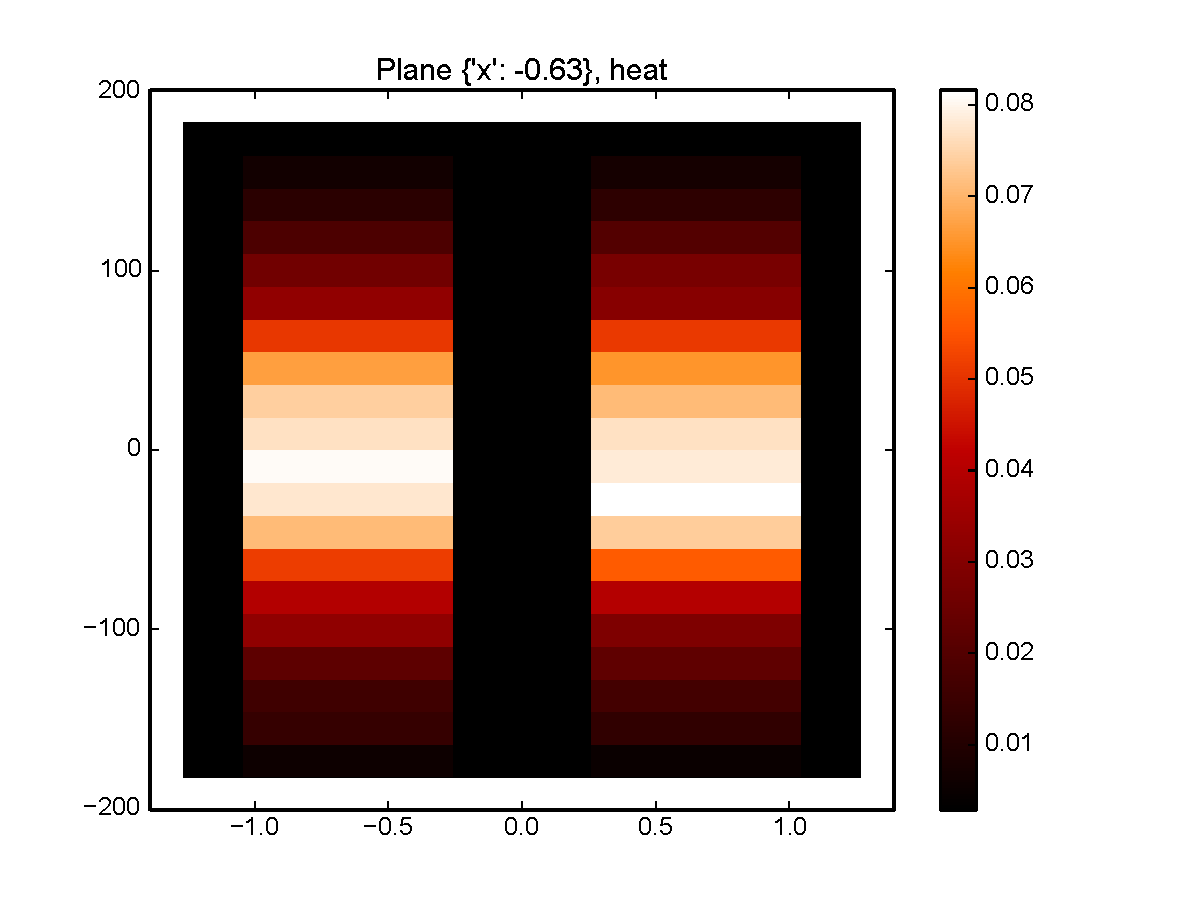
\includegraphics[width=\textwidth]{examples/hmcnp5_hx1.pdf}
        \column{0.5\textwidth}
        {\tiny x plane at 1}
        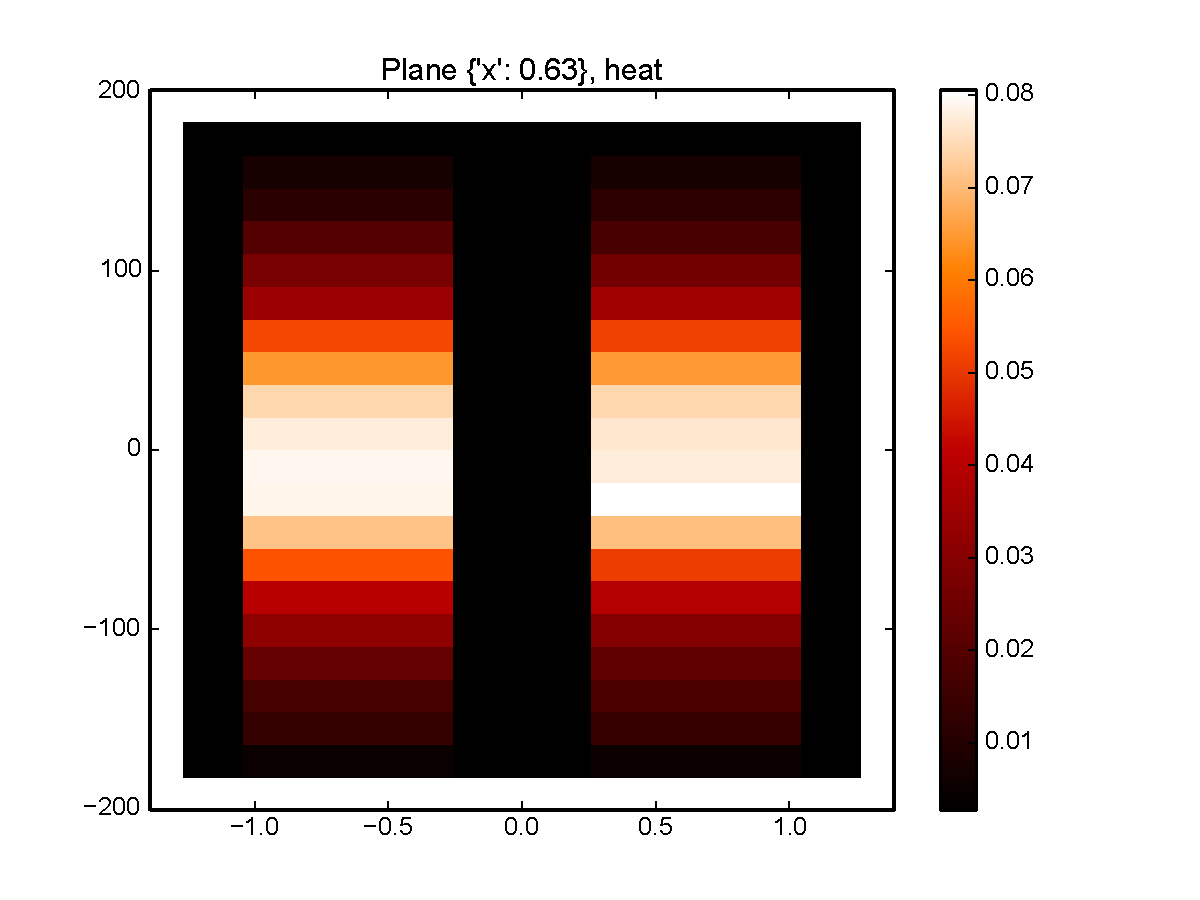
\includegraphics[width=\textwidth]{examples/hmcnp5_hx2.pdf}
    \end{columns}
\end{frame}


